\documentclass[student]{ITRslides}
\usepackage{tikz,pgfplots,epstopdf,psfrag,pstricks}
\pgfplotsset{compat=1.9}
\usepgfplotslibrary{groupplots}
\usetikzlibrary{matrix} 
\addbibresource{../../Thesis/mybib.bib}
\AtEveryBibitem{\clearfield{note}}
\AtEveryBibitem{\clearfield{isbn}}
\AtEveryBibitem{\clearfield{doi}}
\AtEveryBibitem{\clearfield{issn}}
\AtEveryBibitem{\clearname{editor}}
\graphicspath{{pics/}{logos/}}
\newcommand{\f}[1]{\boldsymbol{#1}}
\newcommand{\g}[1]{\text{#1}}

\title{Control of a multi-robot cooperative team guided by a human operator}
\presenter{M. Angerer}

\supervisor{S. Musi\'c}
\typeofpres{Final Presentation Master Thesis}

\usetikzlibrary{decorations.pathreplacing}
\newcommand{\tikzmark}[2]{\tikz[remember picture,baseline=(#1.base)]{\node[inner sep=0pt] (#1) {#2};}}
%%%%%%%%%%%%%%%%%%%%%%%%%%%%%%%%%%%%%%%%%%%%%%%%%%%%%%%%%%%%%%%%%%%%%%%%%%%%%%%%

\begin{document}


\begin{frame}
    \titlepage
\end{frame}

%\begin{frame}
%	\frametitle{Overview}
%    \tableofcontents%[hideallsubsections]%[pausesections]
%\end{frame}

\section{Introduction}

\begin{frame}
	\frametitle{Shared control with a human in the loop}
	Human reasoning combines with the enhanced flexibility of multiple robots 
		\begin{columns}[T]
		\column{0.5\linewidth}
	
			\begin{figure}
			\centering
			%\psfrag{q1}[Bl][Bl]{\small $\alpha$}
			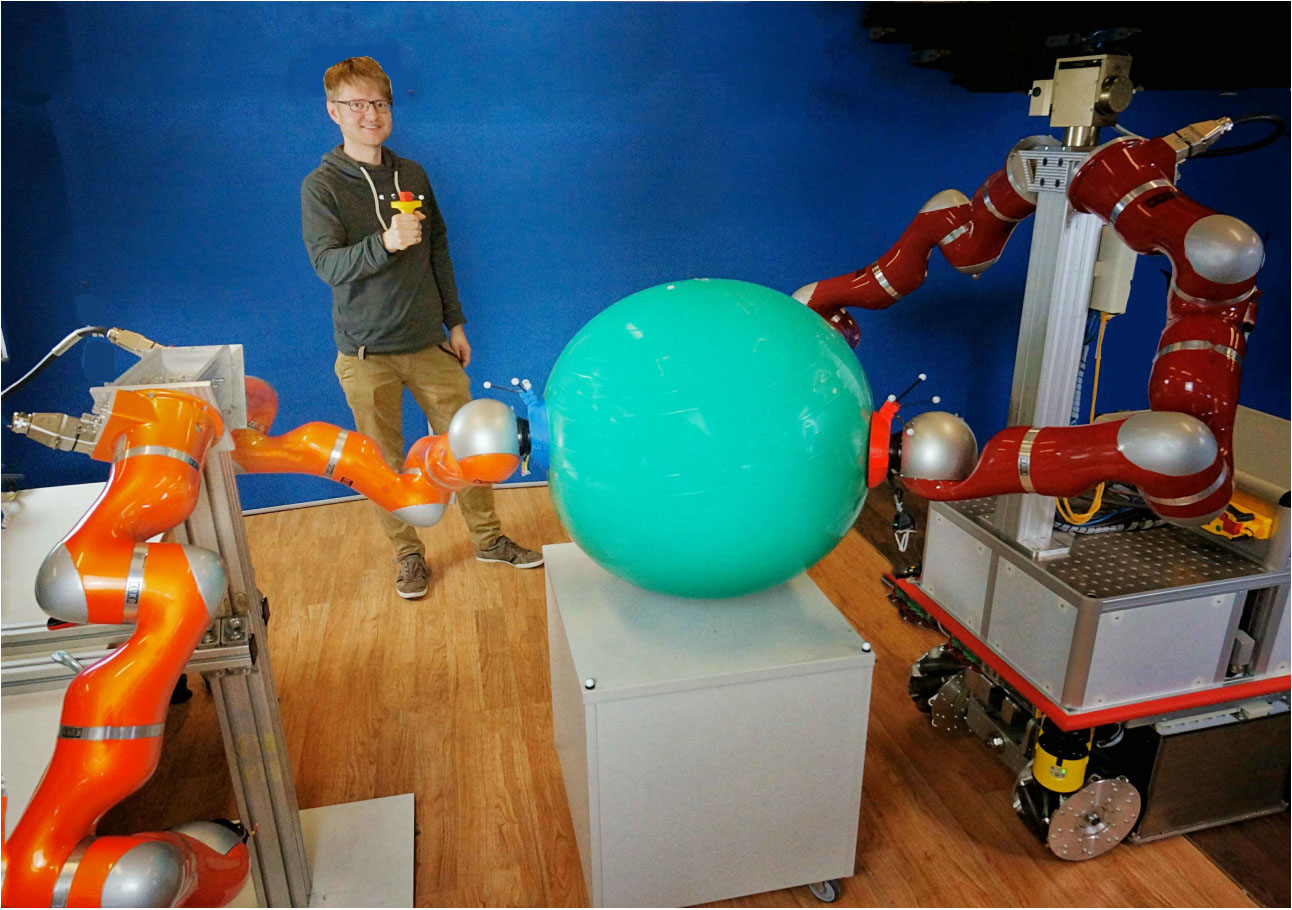
\includegraphics[width=0.98\textwidth]{handcontrol.jpg}
			%\caption{Coordinated handling of tools by a tele-operated robot \cite{MHI-MEISTeR}}
			\end{figure}
		
		\column{0.5\linewidth}
		\vspace{10pt}
		Non-restrictive input interfaces allow for almost arbitrary trajectories\\
		\begin{block}{}
			\textit{How can we ensure stability and safety with a human in the loop?}
		\end{block}
		
			
			\end{columns}
\end{frame}

\begin{frame}
	\frametitle{Problem setting}
		\begin{columns}
%	\begin{itemize}
%		\item Precise and stable control during free-motion/contact transition
%		\item Enhance versatility by performing friction grasps
%		\item (Intuitive) high-level human shared control
%		\item Local control of formation, independent of the operator
%		\item Assistance of the operator with suitable feedback
%	\end{itemize}
	\column{0.5\linewidth}
	\begin{itemize}
	\item A set of robots manipulating a common object
	\item A human guiding the formation by hand motion
	\end{itemize}
		
	\column{0.5\linewidth}
	
	
			\begin{figure}
			\centering
			%\psfrag{q1}[Bl][Bl]{\small $\alpha$}
			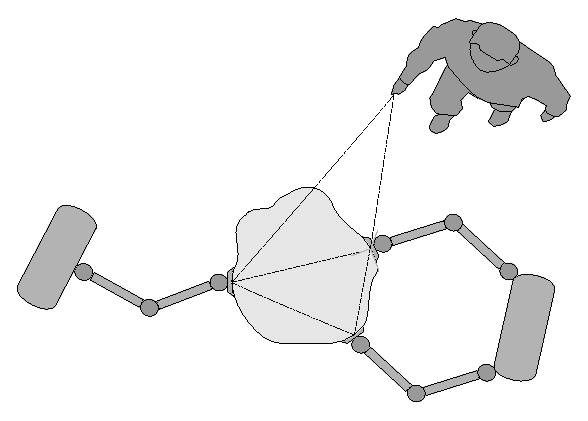
\includegraphics[width=0.8\textwidth]{general_setup.eps}

			\end{figure}
	\end{columns}
	\vspace{10pt}
	\begin{block}{Goals for control design}
	\begin{itemize}
	\item Automatic preservation of formation 
	\item Stability with arbitrary trajectories
	\item Safe behaviour with humans on-site
	\end{itemize}
	\end{block}	

\end{frame}

\begin{frame}
	\frametitle{Related Work}
	\textbf{Robot-team control}
	\begin{itemize}
		\item (Inverse) grasp-matrix approaches \nocite{Schneider_92,Caccavale_08} {\tiny [SC92,CCMV08]} 	
		\item Virtual structures \nocite{Stramigioli_01, Sieber_15} {\tiny [Str01,SMH15]} 
	\end{itemize}
	\textbf{Human in the loop}
	\begin{itemize}	
		\item Bilateral tele-manipulation  \nocite{Lee_05} {\tiny [LS05]} 	
		\item Human leader - robotic followers \nocite{Sieber_15, Scheggi_14}{\tiny [SMH15,SMP14]} 
		\item Gesture-based Control \nocite{Gioioso_2014}{\tiny [GFS+14]} 
	\end{itemize}
	\textbf{Safety by energy-regulation}
	\begin{itemize}
		\item Adaptive impedance control of a single manipulator \nocite{Tadele_14}{\tiny [TVS14]}
		\item Energy observer in physical human-robot interaction \nocite{Geravand_16}{\tiny [GSLP16]}
	\end{itemize}
		
			\begin{block}{}
			\begin{itemize}
			\item Stability with non-restrictive input interfaces is unexplored
			\item Passivity is commonly used to cope with unmodelled dynamics

			\item Energy-based safety metrics apply for impact limitation 
			\end{itemize}
			\end{block}
\end{frame}

%\begin{frame}
%	\frametitle{Related Work: Human in the loop}
%	\begin{itemize}	
%		\item Formation-based control \nocite{Sieber_15, Scheggi_14}{\tiny [SMH15,SMP14]} 
%%		\begin{itemize}
%%			\item Single leader, multiple followers
%%			\item Robots preserve formation autonomously
%%			\item Tactile feedback
%%		\end{itemize}
%		\item Bilateral tele-manipulation  \nocite{Lee_05} {\tiny [LS05]} 
%%		\begin{itemize}
%%			\item Single master coupled to human, constrained system as slave
%%			\item Local control of interaction dynamics
%%			\item Force feedback
%%		\end{itemize}
%
%		\item Gesture-based Control \nocite{Gioioso_2014}{\tiny [GFS+14]} 
%%		\begin{itemize}
%%			\item Free-hand motion controls constrained system
%%			\item Visual feedback
%%			%\item only visual feedback
%%		\end{itemize}
%		\end{itemize}
%		
%			\begin{block}{}
%			\begin{itemize}
%			\item port-Hamiltonian systems allow for energy consistent modelling of complex physical systems
%			\item \emph{IPC} concept based on a physical model
%
%			\item Closed loop stability for bounded energy supply% and a passive control architecture
%			\end{itemize}
%
%	\end{block}
%	
%\end{frame}

\section{Approach}

%\begin{frame}
%	\frametitle{port-Hamiltonian systems}
%\emph{Hamiltonian} equations of a mechanical system
%\[ \dot{q} = \frac{\partial H}{\partial p}(q,p) \]
%\[\dot{p} = -\frac{\partial H}{\partial q}(q,p) + F \]
%\emph{Hamiltonian} $ H(q,p)$: total energy\\
%generalized coordinates $q$, generalized momenta $p$, external generalized forces $F$
% 
%\textbf{Energy balance}
%\[ \frac{d}{dt} H = \frac{\partial^T H}{\partial q} \dot{q} + \frac{\partial^T H}{\partial p}\dot{p} = \frac{\partial^T H}{\partial p} F = \dot{q}^T F \]
%
%\end{frame}


\begin{frame}
	\frametitle{Overview}
	
	\begin{figure}
		\centering
		%\psfrag{q1}[Bl][Bl]{\small $\alpha$}
		\def\svgwidth{0.99\columnwidth}
		\input{pics/overview.eps_tex}
	\end{figure}
	\begin{itemize}
		\item Source for the passive robot-team controller: Energy Tank
		\item Human user controls the power flow
		\item Energy supplied to the robots is re-fed into the tank
	\end{itemize}
	\begin{block}{}
		Energy-consistent description in the \emph{port-Hamiltonian} framework
		\end{block}
	
\end{frame}


\begin{frame}
	\frametitle{port-Hamiltonian systems}
	\begin{block}{}
	Visualize power flow, allow for model-based control design,\\ facilitate stability proofs
	\end{block}	
	\textbf{Hamiltonian} $\mathcal{H}$: total energy of the system\\
		\textbf{Port}: power-conjugated pair $(u,y)$ of \emph{flow} $u$ and \emph{effort} $y$ variables\\
	\begin{align*}
		 \dot{x} &= \left[J(x)-R(x)\right]\frac{\partial \mathcal{H}}{\partial x}(x) +B(x)u \\
y &= B^T(x)\frac{\partial \mathcal{H}}{\partial x}(x)
	\end{align*}

	input-state-output form with \emph{structure-} $J(x)$, \emph{dissipation-} $R(x)$\\ and \emph{mapping }matrix $B(x)$ \\

	\textbf{Energy balance:}  $ \frac{d}{dt}\mathcal{H} = y^Tu - \frac{\partial^T \mathcal{H}}{\partial x}R(x)\frac{\partial \mathcal{H}}{\partial x} $ ($\rightarrow$ passive)
	
	

%	\begin{itemize}
%	
%		\item Mechanical energy storing elements (spring, mass)
%		\item Dissipation element (Damper)
%		\item Conservative elements (transformer, gyrator)
%		\item Interconnection: power port $ \mathcal{P} = \mathcal{V} \times \mathcal{V}^* $ \\ $\mathcal{V}$: space of efforts; $\mathcal{V}*$: (dual) space of flows
%		\end{itemize}
%		\textit{Example:} Inertia
%\[
%	\dot{P^b} = C_b \frac{\partial H(P^b)}{\partial P^b} +  W^b \]
%	\[T_b^{b,0} = \frac{\partial H(P^b)}{\partial P^b}
%\]
%$H = \frac{1}{2} (P^b)^T M_b^{-1} P^b$: kinetic energy;\\ $P^b$: momentum (state); $T_b^{b,0}$: twist (effort); $W^b$: wrench (flow)
		
		
%		\[\begin{pmatrix}\dot{x}_B \\ \dot{x}_S\end{pmatrix} = 
%		\begin{pmatrix}J_B & -Ad_{H_b^0}^T \phi_b^T \\ \phi_b Ad_{H_b^0} & 0\end{pmatrix}
%		\begin{pmatrix}\frac{\partial V}{\partial x_B} \\ \frac{\partial V}{\partial x_S}\end{pmatrix} + \begin{pmatrix}0 & 0 & 0 \\ \phi_v & \phi_i & \phi_{rl}\end{pmatrix}	
%		\begin{pmatrix}T_v^0 \\ T_i^0 \\ T_{rl}^b\end{pmatrix}			 \]
%		\[\begin{pmatrix}W_v^0 \\ W_i^0 \\ W_{rl}^b\end{pmatrix}=
%		\begin{pmatrix}0 & \phi_v^T\\0 & \phi_i^T\\0 & \phi_{rl}^T	
%		\end{pmatrix}
%		\begin{pmatrix}\frac{\partial V}{\partial x_B} \\ \frac{\partial V}{\partial x_S}\end{pmatrix}\]
%		\item Conservative elements (transformer, gyrator)
%			\item Interconnection through power ports
%		\[ \mathcal{P} = \mathcal{V} \times \mathcal{V}^* \]
%		\item Example: variable rest-length spring
%		\begin{eqnarray}\label{EQ:variablerestlengthspring}
%	\dot{H}_i^j =\left( \begin{pmatrix}1 & Ad_{H_b^j}\end{pmatrix} \begin{pmatrix}T_b^{j} \\ T_i^{b}\end{pmatrix} \right) H_i^j\\
%	\begin{pmatrix}W_b^{j,j} \\ W_i^{b,b}\end{pmatrix}  = \left( \begin{pmatrix}1 \\ Ad_{H_b^j}^T\end{pmatrix} \frac{\partial V_{i,j}}{\partial H_i^j} \right) (H_i^j)^T
%\end{eqnarray}

%\end{itemize}

\end{frame}

\begin{frame}
	\frametitle{Model-based control design}
	\textit{Plants and controllers are energy-transforming devices, which we interconnect to achieve the desired behaviour.} \nocite{Ortega_01}{\tiny [OSMM01]}
	\vspace{10pt}
		\begin{columns}
			\column{0.4\linewidth}
			\begin{figure}
			\centering
			%\psfrag{q1}[Bl][Bl]{\small $\alpha$}
			\def\svgwidth{1\columnwidth}
			\input{pics/virtualstructure.eps_tex}
			\end{figure}
			\column{0.6\linewidth}
			\textbf{Virtual structure}
			\begin{itemize}
				\item Geometric composition of springs, masses and dampers
				\item Establishing a formation of robots
				\item Virtually coupling the human
				\item Energetic model of the real system
				\item Connection by physical rules \\ (actio = reactio) 
			\end{itemize}
			\end{columns}
								\begin{block}{Stability}
									Model errors never influence passivity nor stability \nocite{Stramigioli_01}{\tiny [Str01]} 
								\end{block}

\end{frame}

%\begin{frame}
%	\frametitle{Energy consistent modelling and control}
%	\begin{itemize}
%		\item \emph{Virtual object} concept
%			\begin{itemize}%[leftmargin=0em]
%  				\renewcommand{\labelitemi}{$\Rightarrow$}
%				\item Maps object forces to manipulators
%				\item Stores kinetic energy
%				\item Changes size to adjust formation
%			\end{itemize}
%		\item Model represents energy content of the complete system
%		\item Dampers dissipate energy: \textbf{passive system}
%		\item Operator controls system by energy supply
%			\begin{block}{Stability}
%Model errors never influence passivity nor stability \cite{Stramigioli_01}
%	\end{block}	
%		\end{itemize}
%%\begin{itemize}%[leftmargin=0em]
%%  \renewcommand{\labelitemi}{$\Rightarrow$}
%%\item enhanced human perception through control of a meaningful quantity and appropriate feedback
%%\item stability over a wide class of environments
%%			\end{itemize}
%%		\begin{quote}
%%		If a controlled robot is not passive there is always a passive environment that destabilizes the interconnected system \cite{Stramigioli_15}
%%		\end{quote}
%
%
%\end{frame}


%\begin{frame}
%	\frametitle{Intrinsically Passive Control (IPC)}
%	\begin{columns}
%		\column{0.4\linewidth}
%			
%	
%		\begin{itemize}
%			\item High-level Supervisor and low-level IPC
%			\item IPC + robot: passive
%			\item Power provided by Supervisor
%			\item Environment assumed passive
%		\end{itemize}
%
%		
%		\column{0.58\linewidth}
%             \begin{figure}[htb]
%			\centering
%			%\psfrag{q1}[Bl][Bl]{\small $\alpha$}
%			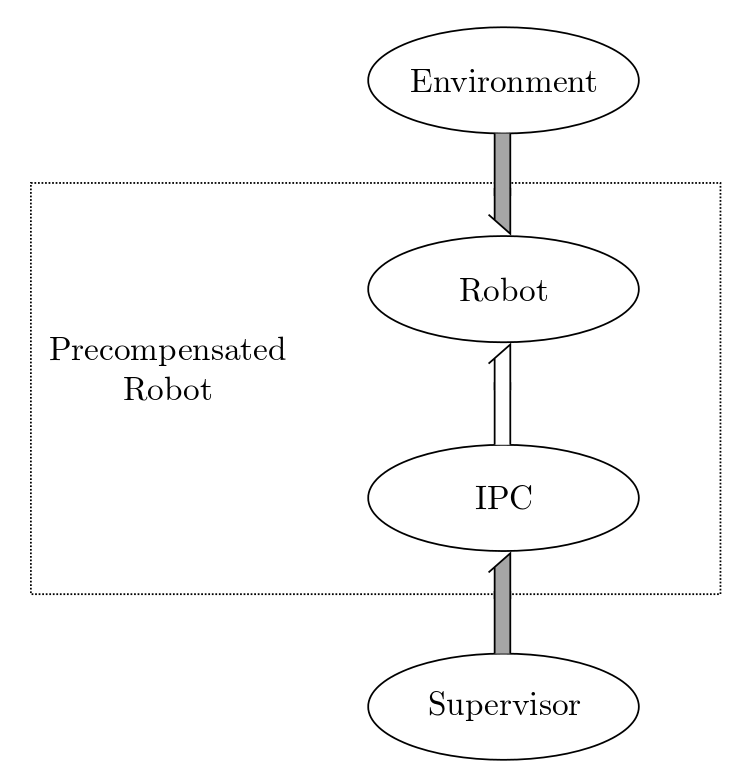
\includegraphics[width=0.9\textwidth]{IPCoverview.png}
%			\caption{Overview of the IPC architecture 								\cite{Stramigioli_01}}
%			\end{figure}
%		
%			
%		\end{columns}
%\end{frame}

\begin{frame}
	\frametitle{Example controller derivation}
\only<1>{Starting from the virtual object...
	 \[
	\begin{aligned}
	&\dot{P_b^b} = C_b \frac{\partial \mathcal{H}}{\partial P_b^b} + I_6 W_{b}^b \\
	&T_b^{b,0} = I_6 \frac{\partial \mathcal{H}}{\partial P_b^b}
	\end{aligned}
	\]
	
		\begin{figure}

			%\psfrag{q1}[Bl][Bl]{\small $\alpha$}
			\def\svgwidth{0.1\columnwidth}
			\input{pics/controlderivation1.eps_tex}
		\end{figure}
Momentum $P_b^b$ (state), wrench $W_b^b$ (flow), twist $T_b^{b,0}$ (effort), \\ centripetal and Coriolis terms $C_b$\\ 
\textbf{Hamiltonian} $\mathcal{H}= \frac{1}{2} {P_b^b}^T M_b^{-1} P_b^b$}


%\end{frame}
%
%\begin{frame}
	%\frametitle{Example controller derivation}
\only<2>{	... adding a coupling spring to the user...
	\[
	\begin{aligned}
	&\begin{pmatrix}\dot{H}_b^v \\ \dot{P_b^b} \end{pmatrix}=
	\begin{pmatrix} 0 & H_b^v \\ -{H_b^v}^T & C_b \end{pmatrix}
	\begin{pmatrix} \frac{\partial \mathcal{H}}{\partial H_b^v} \\ \frac{\partial \mathcal{H}}{\partial P_b^b}  \end{pmatrix} + 
	\begin{pmatrix} -H_b^v Ad_{H_0^b} & 0 \\ 0 & I_6\end{pmatrix} 
	\begin{pmatrix} T_v^0 \\ W_{b}^b \end{pmatrix}\\
	& \begin{pmatrix}
	W_v^0 \\ T_b^{b,0} \end{pmatrix} = 
	\begin{pmatrix}	-Ad_{H_0^b}^T {H_b^v}^T & 0 \\ 0 & I_6	\end{pmatrix}
	\begin{pmatrix} \frac{\partial \mathcal{H}}{\partial H_b^v} \\ \frac{\partial \mathcal{H}}{\partial P_b^b}  \end{pmatrix}
	\end{aligned}
	\]
	
	\begin{figure}
		
		%\psfrag{q1}[Bl][Bl]{\small $\alpha$}
		\def\svgwidth{0.25\columnwidth}
		\input{pics/controlderivation2.eps_tex}
	\end{figure}
	relative configuration $H_b^v$ (state), desired twist $T_v^0$ (flow),\\ wrench $W_v^0$ (effort), adjoint mapping $Ad_{H_0^b}$\\ 
	\textbf{Hamiltonian} $\mathcal{H}= \frac{1}{2} {P_b^b}^T M_b^{-1} P_b^b + V_\g{P}(H_b^v)$}
	
	
%\end{frame}
%
%\begin{frame}
%	\frametitle{Example controller derivation}
\only<3>{... and another spring to the $i$-th manipulator.
	\resizebox{1\vsize}{!}{$
		\begin{aligned}
	\begin{pmatrix}\dot{H}_b^v \\ \dot{P_b^b} \\ \dot{H}_{b(i)}^i\end{pmatrix}&=
	\begin{pmatrix} 0 & H_b^v & 0 \\ -{H_b^v}^T & C_b & -Ad_{H_b^{b(i)}}^T {H_{b(i)}^i}^T \\ 0 & H_{b(i)}^i Ad_{H_b^{b(i)}} & 0 \end{pmatrix}
	\begin{pmatrix} \frac{\partial \mathcal{H}}{\partial H_b^v} \\ \frac{\partial \mathcal{H}}{\partial P_b^b} \\ \frac{\partial \mathcal{H}}{\partial H_{b(i)}^i}  \end{pmatrix} \\ 
	&+ 
	\begin{pmatrix} -H_b^v Ad_{H_0^b} & 0 \\ 0 & 0 \\ 0 & -H_{b(i)}^i Ad_{H_0^{b(i)}}\end{pmatrix} 
	\begin{pmatrix} T_v^0 \\ T_i^0 \end{pmatrix}\\
	 \begin{pmatrix}
	W_v^0 \\ W_i^0 \end{pmatrix} &= 
	\begin{pmatrix}	-Ad_{H_0^b}^T {H_b^v}^T & 0 & 0\\ 0 & 0 & -Ad_{H_0^{b(i)}}^T {H_{b(i)}^i}^T	\end{pmatrix}
	\begin{pmatrix} \frac{\partial \mathcal{H}}{\partial H_b^v} \\ \frac{\partial \mathcal{H}}{\partial P_b^b} \\ \frac{\partial \mathcal{H}}{\partial H_{b(i)}^i}  \end{pmatrix} \\
	\end{aligned}
	$}
	
	\begin{figure}
		
		%\psfrag{q1}[Bl][Bl]{\small $\alpha$}
		\def\svgwidth{0.4\columnwidth}
		\input{pics/controlderivation3.eps_tex}
	\end{figure}
	\textbf{Hamiltonian} $\mathcal{H}= \frac{1}{2} {P_b^b}^T M_b^{-1} P_b^b + V_\g{P}(H_b^v) + V_\g{P}(H_{b(i)}^i)$}
	
\end{frame}

\begin{frame}
	\frametitle{Modelling of rigid contact}
	In cooperative manipulation it is common to assume a rigid connection of manipulators and object. \\
	\textbf{Kinematic constraints} $ 0 = A^T(x)\frac{\partial \mathcal{H}}{\partial x}$ ($\rightarrow$ DAEs)\\
	
	\begin{block}{Solved input-state-output form}
		\resizebox{!}{!}{$
			\begin{aligned}
			\dot{x} &= \left[J(x)-R(x)\right]\frac{\partial \mathcal{H}}{\partial x}(x) +B(x)u\\ &+ A(A^TM^{-1}A)^{-1} A^T M^{-1} (u+C\frac{\partial \mathcal{H}}{\partial x})\\
			y &= B^T(x)\frac{\partial \mathcal{H}}{\partial x}(x)
			\end{aligned}
		$}
	\end{block}
	Constraint matrix $A$, inertia matrix $M$, centripetal force matrix $C$ \\
	\vspace{6pt}
Rigid connections are power-conservative.\nocite{Schaft_13}{\tiny [Sch13]}

\end{frame}


\begin{frame}
	\frametitle{Energy tanks}
	\textbf{Virtual storage element:} Energy function $\mathcal{T}(x_\g{t}) = \frac{1}{2}x_\g{t}^2$
	\begin{align*}
	x_\g{t} &= u_\g{t} \\
	y_\g{t} &= \frac{\partial \mathcal{T}(x_\g{t})}{\partial x_\g{t}} (=x_\g{t})
	\end{align*}
	Interconnection of tank and controller by a transformer/gyrator
	\begin{align*}
		u = ny_\g{t}\\
		u_\g{t} = -n^T y
	\end{align*}
	The interconnection is power-continuous for any ratio $n$\\
	For $ n = \frac{w}{x_\g{t}}$, $w$ is the new control input
	\begin{align*}
	\dot{x} &= \left[J(x)-R(x)\right]\frac{\partial \mathcal{H}}{\partial x}(x) +B(x)\frac{w}{\color{gray}{x_\g{t}}}{\color{gray}y_\g{t}} \\
	y &= B^T(x)\frac{\partial \mathcal{H}}{\partial x}(x)
	\end{align*} 
\end{frame}


\begin{frame}
	\frametitle{Re-filling and energy balance}
	\begin{figure}[b!]
		\centering
		\footnotesize
		\def\svgwidth{0.95\columnwidth}
		\input{pics/energytank.eps_tex}				
	\end{figure}
	\textit{Lossy robots and unknown energy exchange with the environment}
	Controller dissipation and power supplied to the robots is re-fed into the tank, i.e. $\dot{\mathcal{T}}(x_\g{t})+\dot{\mathcal{H}}=0$.
	\[
	\dot{\mathcal{T}}(x_\g{t}) + \underbrace{\frac{\partial^T \mathcal{H}}{\partial x}R(x)\frac{\partial \mathcal{H}}{\partial x} + \sum_{i=1}^n {W_i^{0}}^T T_i^0}_{\text{compensation}} = - \dot{{\mathcal{H}}} + \sum_{i=1}^n {W_i^{0}}^T T_i^0
	\] 
\end{frame}

\begin{frame}
	\frametitle{Safety metrics and adaptive stiffness}
	Minimal kinetic energies that result in severe injuries \nocite{Tadele_14}{\tiny TVS14}
	\[
	V_{\g{K,min}} = 
	\begin{cases}
	517 \text{ J} & \text{adult cranium bone failure} \\
	127 \text{ J} & \text{infant cranium bone failure} \\
	30 \text{ J} & \text{neck fracture}
	\end{cases}
	\]
	\textit{How can we change user commands to comply with these limits?}
	Human hand is stiff when moving slow, compliant when fast \nocite{Hogan_84b}{\tiny [Hog84]}
	\textbf{Energy-adapted human coupling:} reduced stiffness $\kappa$ and damping below a threshold tank level $\mathcal{T}_{\g{th}}$
	\[
	\kappa = \begin{cases}
	k_{vb} & \text{if } \, \mathcal{T}(x_\g{t})\geq \mathcal{T}_{\g{th}} \\
	k_{vb} \frac{\mathcal{T}(x_\g{t})}{\mathcal{T}_{\g{th}}} & \text{if } \, \mathcal{T}(x_\g{t}) < \mathcal{T}_{\g{th}}
	\end{cases} \]
	\end{frame}




\section{Results}
%\begin{frame}
%	\frametitle{Grasping force optimization for friction contacts}
%	\begin{columns}
%	\column{0.6\textwidth}
%	\begin{itemize}
%	\item required contact normal force is dependent on tangential forces
%	\item high tangential forces arise during acceleration
%	\item other requirements: safety margin, maximum grasping force $\Rightarrow$ cost function
%	\item linear matrix inequality (LMI) problem
%	\end{itemize}
%	\column{0.5\textwidth}
%
%\begin{figure}[htb]
%			\centering
%			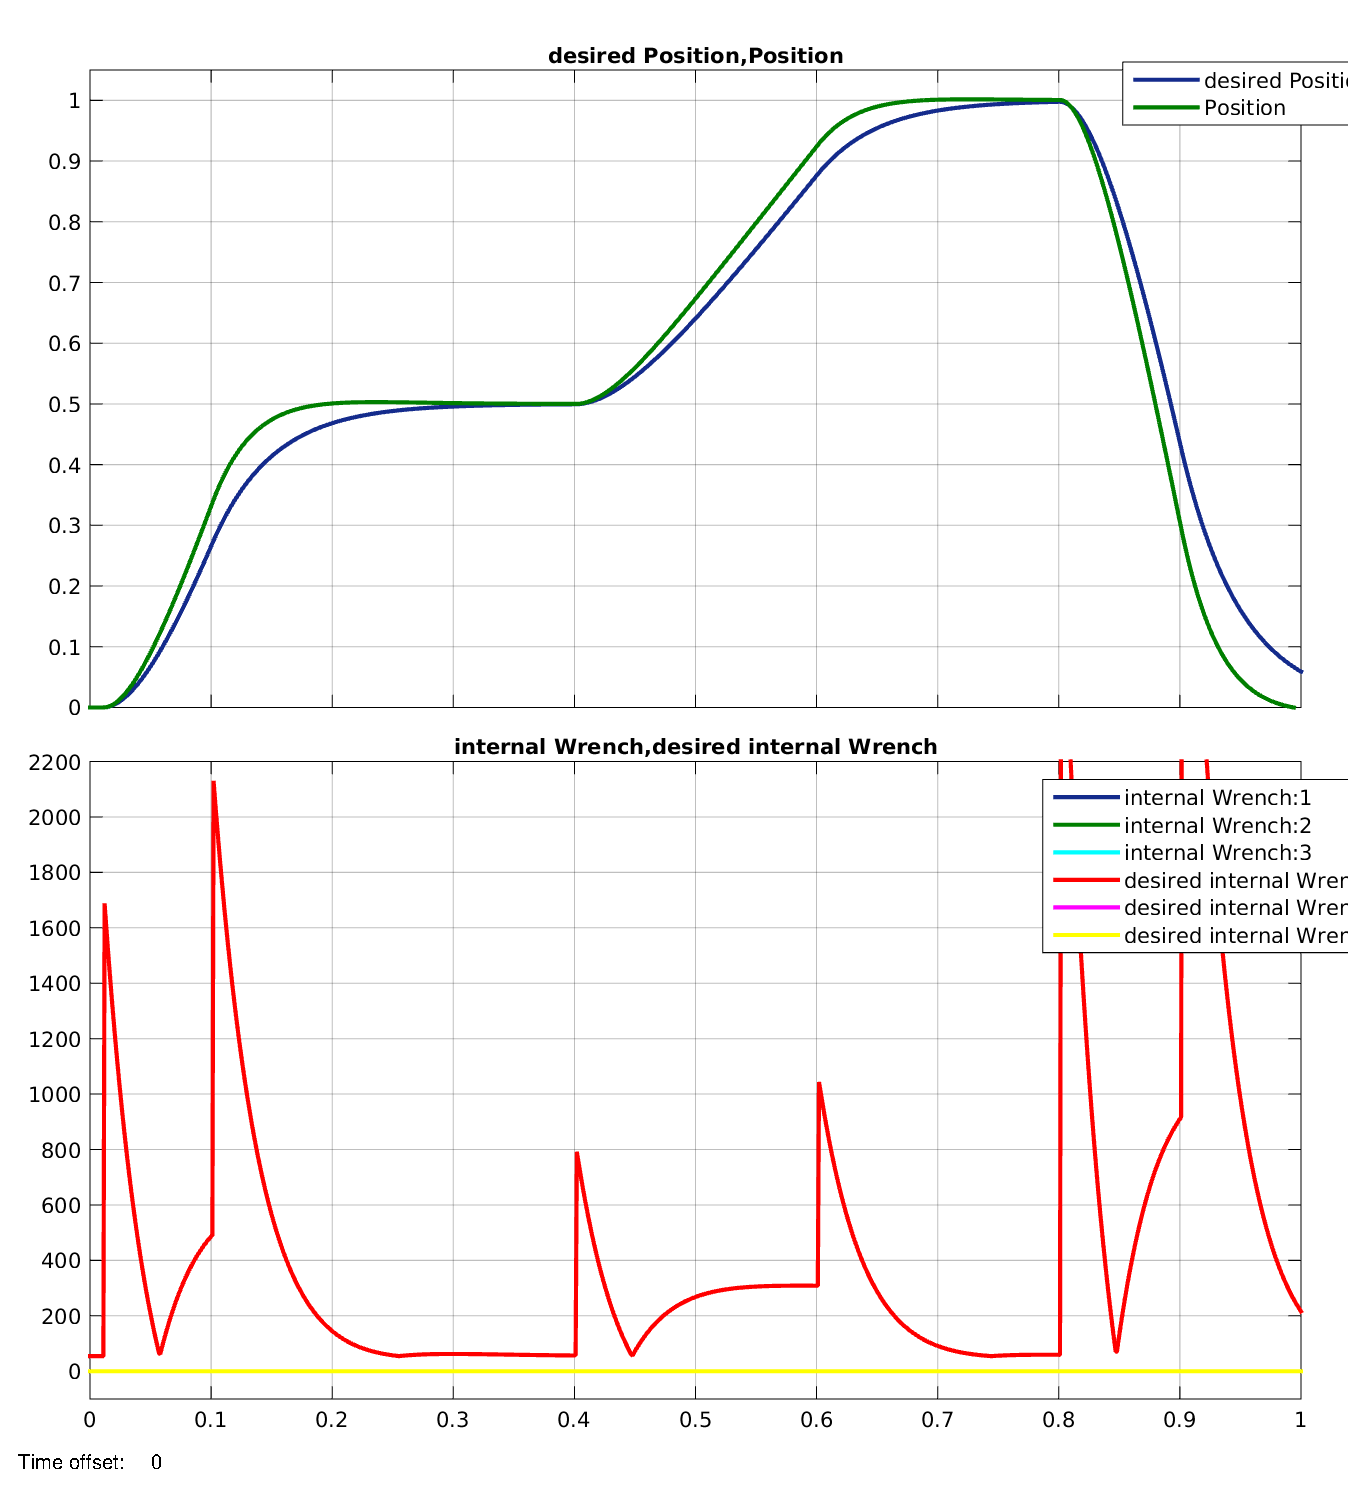
\includegraphics[width=0.9\textwidth]{Hanposforce.eps}
%			\caption{Position, Internal wrench}
%\end{figure}
%\end{columns}
%\end{frame}
\begin{frame}
	\frametitle{Trajectory tracking: Constrained dynamic IPC }
	%\frametitle{Trajectory tracking: Comparison}
	\vspace{-30pt}
	\begin{figure}
%\begin{tikzpicture}
\begin{groupplot}[
      group style={group size=2 by 3,ylabels at=edge left},
      ylabel style={text height=0.02\textwidth,inner ysep=-5pt},
      grid=major,height=0.31\linewidth,width=0.5\linewidth,/tikz/font=\tiny
    ]
    \nextgroupplot[ylabel={Position $p_x$[m]}]
    \addplot[black,] table {../../plotdata/CaVitrans_desired position.txt}; 
	\addplot[blue,] table {../../plotdata/DIPCctrans_position.txt};
	\addplot[green,] table {../../plotdata/StrIPCtrans_position.txt};
	\addplot[red,] table {../../plotdata/CaVitrans_position.txt};
	\coordinate (top) at (rel axis cs:0,1);% coordinate at top of the first plot
	\nextgroupplot[ylabel={Orient. $\Phi_z$[rad]}]
	\addplot[black,] table {../../plotdata/CaVirot_desired Orientation.txt};
	\addplot[blue,] table {../../plotdata/DIPCcrot_Orientation.txt};
	\addplot[red,] table {../../plotdata/CaVirot_Orientation.txt};
	\addplot[green,] table {../../plotdata/StrIPCrot_Orientation.txt};
	\coordinate (bot) at (rel axis cs:1,0);% coordinate at bottom of the last plot
  \end{groupplot}
  % legend
  \path (top|-current bounding box.north)--
        coordinate(legendpos)
        (bot|-current bounding box.north);
  \matrix[
      matrix of nodes,
      anchor=south,
      draw,
      inner sep=0.2em,
    ]at([yshift=1ex]legendpos)
    {	{\color{black}\textemdash} &{desired traj.}&[3pt]
	    {\color{blue}\textemdash} &{constrained dIPC}&[3pt]
      {\color{red}\textemdash} &{impedance ctrl}&[3pt]
      {\color{green}\textemdash} &{dyn. IPC}&[3pt]\\};      
\end{tikzpicture} 
\begin{tikzpicture}
\hspace{3pt}
\begin{groupplot}[
      group style={group size=2 by 3,ylabels at=edge left},
      ylabel style={text height=0.02\textwidth,inner ysep=-5pt},
      grid=major,height=0.31\linewidth,width=0.5\linewidth,/tikz/font=\tiny
    ]
    \nextgroupplot[ylabel={Lin. vel. $\dot{p}_x$[m/s]}] 
    \addplot[black,] table {../../plotdata/CaVitrans_desired velocity.txt};
	\addplot[blue,] table {../../plotdata/DIPCctrans_Velocity.txt};
	\addplot[red,] table {../../plotdata/CaVitrans_Velocity.txt};
	\addplot[green,] table {../../plotdata/StrIPCtrans_Velocity.txt};
	\coordinate (top) at (rel axis cs:0,1);% coordinate at top of the first plot
	\nextgroupplot[ylabel={Ang. vel. $\omega_z$[rad/s]}]
	\addplot[black,] table {../../plotdata/CaVirot_desired ang velocity.txt};
	\addplot[blue,] table {../../plotdata/DIPCcrot_Angular Velocity.txt};
	\addplot[red,] table {../../plotdata/CaVirot_Angular Velocity.txt};
	\addplot[green,] table {../../plotdata/StrIPCrot_Angular Velocity.txt};
	\coordinate (bot) at (rel axis cs:1,0);% coordinate at bottom of the last plot
  \end{groupplot}
  % legend
%  \path (top|-current bounding box.north)--
%        coordinate(legendpos)
%        (bot|-current bounding box.north);
%  \matrix[
%      matrix of nodes,
%      anchor=south,
%      draw,
%      inner sep=0.2em,
%    ]at([yshift=1ex]legendpos)
%    { \ref*{plots:errVeloc}&{ $\Delta\dot{p}_x$ [m/s]}&[5pt]
%      \ref*{plots:errAngVel}&{ $\Delta\omega_z$ [rad/s]}&[5pt]\\};
\end{tikzpicture}
\begin{tikzpicture}
\begin{groupplot}[
	group style={group size=2 by 3,ylabels at=edge left},
	ylabel style={text height=0.02\textwidth,inner ysep=-10pt},
	grid=major,height=0.31\linewidth,width=0.5\linewidth,/tikz/font=\tiny
	]
	\nextgroupplot[xlabel={$t$[s]}, ylabel={Force $f_x$[N]}] 
	\addplot[blue,] table {../../plotdata/DIPCctrans_Manipulator wrench_tx.txt};
	\addplot[red,] table {../../plotdata/CaVitrans_Manipulator wrench_tx.txt};
	\addplot[green,] table {../../plotdata/StrIPCtrans_Manipulator wrench_tx.txt};
	\coordinate (top) at (rel axis cs:0,1);% coordinate at top of the first plot
	\nextgroupplot[xlabel={$t$[s]}, ylabel={Force $f_y$[N]}]
	\addplot[blue,] table {../../plotdata/DIPCcrot_Manipulator wrench_ty.txt};
	\addplot[red,] table {../../plotdata/CaVirot_Manipulator wrench_ty.txt};
	\addplot[green,] table {../../plotdata/StrIPCrot_Manipulator wrench_ty.txt};
	\coordinate (bot) at (rel axis cs:1,0);% coordinate at bottom of the last plot
\end{groupplot}
\end{tikzpicture} 

%\begin{tikzpicture}
%\begin{groupplot}[
%      group style={group size=2 by 3,ylabels at=edge 			left},
%      ylabel style={text height=0.02\textwidth,inner 			ysep=0pt},
%      grid=major,height=0.35\linewidth,width=0.495\linewidth,/tikz/font=\small
%    ]
%    \nextgroupplot[ylabel={Manipulator wrench}]  
%	\addplot[red,] table {../../plotdata/DIPCctrans_Manipulator wrench_tx.txt}; 
%	\addplot[blue,] table {../../plotdata/DIPCctrans_Manipulator wrench_ty.txt}; 
%	\addplot[green,] table {../../plotdata/DIPCctrans_Manipulator wrench_rz.txt};	
%	\coordinate (top) at (rel axis cs:0,1);% coordinate at top of the first plot
%	\nextgroupplot
%	\addplot[red,] table {../../plotdata/DIPCcrot_Manipulator wrench_tx.txt};\label{plots:forcex}
%	\addplot[blue,] table {../../plotdata/DIPCcrot_Manipulator wrench_ty.txt};\label{plots:forcey} 
%	\addplot[green,] table {../../plotdata/DIPCcrot_Manipulator wrench_rz.txt};\label{plots:torquez}	
%	\coordinate (bot) at (rel axis cs:1,0);% coordinate at bottom of the last plot
%  \end{groupplot}
%  % legend
%  \path (top|-current bounding box.north)--
%        coordinate(legendpos)
%        (bot|-current bounding box.north);
%  \matrix[
%      matrix of nodes,
%      anchor=south,
%      draw,
%      inner sep=0.2em,
%    ]at([yshift=1ex]legendpos)
%    { \ref*{plots:forcex}&{ $f_x$ [N]}&[5pt]
%    	  \ref*{plots:forcey}&{ $f_y$ [N]}&[5pt]
%      \ref*{plots:torquez}&{ $m_z$ [Nm]}&[5pt]\\};
%\end{tikzpicture}



\begin{tikzpicture}
\begin{groupplot}[
      group style={group size=2 by 3,ylabels at=edge 			left},
      ylabel style={text height=0.02\textwidth,inner 			ysep=-5pt},
      grid=major,height=0.3\linewidth,width=0.48\linewidth,/tikz/font=\tiny
    ]
    \nextgroupplot[ylabel={Position $\Delta p_x$[m]}] 
	\addplot[blue,] table {../../plotdata/DIPCctrans_errPos.txt};
	%\addplot[green,] table {../../plotdata/StrIPCtrans_errPos.txt};
	%\addplot[red,] table {../../plotdata/CaVitrans_errPos.txt};
	\coordinate (top) at (rel axis cs:0,1);% coordinate at top of the first plot
	\nextgroupplot[ylabel={Orient. $\Delta \Phi_z$[rad]}]
	\addplot[blue,] table {../../plotdata/DIPCcrot_errOrient.txt};
	%\addplot[red,] table {../../plotdata/CaVirot_errOrient.txt};
	%\addplot[green,] table {../../plotdata/StrIPCrot_errOrient.txt};
	\coordinate (bot) at (rel axis cs:1,0);% coordinate at bottom of the last plot
  \end{groupplot}
%  % legend
%  \path (top|-current bounding box.north)--
%        coordinate(legendpos)
%        (bot|-current bounding box.north);
%  \matrix[
%      matrix of nodes,
%      anchor=south,
%      draw,
%      inner sep=0.2em,
%    ]at([yshift=1ex]legendpos)
%    { {\color{blue}\textemdash} &{constrained IPC}&[3pt]
%      {\color{red}\textemdash} &{classic impedance control}&[3pt]
%      {\color{green}\textemdash} &{classic IPC}&[3pt]\\};
      
\end{tikzpicture} 



\begin{tikzpicture}
\begin{groupplot}[
      group style={group size=2 by 3,ylabels at=edge 			left},
      ylabel style={text height=0.02\textwidth,inner ysep=-5pt},
      grid=major,height=0.3\linewidth,width=0.48\linewidth, /tikz/font=\tiny ]
    \nextgroupplot[ylabel={Lin. vel. $\Delta \dot{p}_x$[m/s]}] 
	\addplot[blue,] table {../../plotdata/DIPCctrans_errVeloc.txt};
	%\addplot[red,] table {../../plotdata/CaVitrans_errVeloc.txt};
	%\addplot[green,] table {../../plotdata/StrIPCtrans_errVeloc.txt};
	\coordinate (top) at (rel axis cs:0,1);% coordinate at top of the first plot
	\nextgroupplot[ylabel={Ang. vel. $\Delta \omega_z$[rad/s]}]
	\addplot[blue,] table {../../plotdata/DIPCcrot_errAngVel.txt};
	%\addplot[red,] table {../../plotdata/CaVirot_errAngVel.txt};
	%\addplot[green,] table {../../plotdata/StrIPCrot_errAngVel.txt};
	\coordinate (bot) at (rel axis cs:1,0);% coordinate at bottom of the last plot
  \end{groupplot}
  % legend
%  \path (top|-current bounding box.north)--
%        coordinate(legendpos)
%        (bot|-current bounding box.north);
%  \matrix[
%      matrix of nodes,
%      anchor=south,
%      draw,
%      inner sep=0.2em,
%    ]at([yshift=1ex]legendpos)
%    { \ref*{plots:errVeloc}&{ $\Delta\dot{p}_x$ [m/s]}&[5pt]
%      \ref*{plots:errAngVel}&{ $\Delta\omega_z$ [rad/s]}&[5pt]\\};
\end{tikzpicture} 



\begin{tikzpicture}
\begin{groupplot}[
      group style={group size=2 by 3,ylabels at=edge 			left},
      ylabel style={text height=0.02\textwidth,inner 			ysep=-5pt},
      grid=major,height=0.3\linewidth,width=0.48\linewidth,/tikz/font=\tiny
    ]
    \nextgroupplot[xlabel={$t$[s]},ylabel={Wrench $f_x$[N]}]  
	\addplot[red,] table {../../plotdata/DIPCctrans_Manipulator wrench_tx.txt}; 
	\addplot[blue,] table {../../plotdata/DIPCctrans_Manipulator wrench_ty.txt}; 
	\addplot[green,] table {../../plotdata/DIPCctrans_Manipulator wrench_rz.txt};	
	\coordinate (top) at (rel axis cs:0,1);% coordinate at top of the first plot
	\nextgroupplot[xlabel={$t$[s]},ylabel={$f_x$[N],$f_y$[N],$m_z$[Nm]}]
	\addplot[red,] table {../../plotdata/DIPCcrot_Manipulator wrench_tx.txt};\label{plots:forcex}
	\addplot[blue,] table {../../plotdata/DIPCcrot_Manipulator wrench_ty.txt};\label{plots:forcey} 
	\addplot[green,] table {../../plotdata/DIPCcrot_Manipulator wrench_rz.txt};\label{plots:torquez}	
	\coordinate (bot) at (rel axis cs:1,0);% coordinate at bottom of the last plot
  \end{groupplot}
%  % legend
%  \path (top|-current bounding box.north)--
%        coordinate(legendpos)
%        (bot|-current bounding box.north);
%  \matrix[
%      matrix of nodes,
%      anchor=south,
%      draw,
%      inner sep=0.2em,
%    ]at([yshift=1ex]legendpos)
%    { \ref*{plots:forcex}&{ $f_x$ [N]}&[5pt]
%    	  \ref*{plots:forcey}&{ $f_y$ [N]}&[5pt]
%      \ref*{plots:torquez}&{ $m_z$ [Nm]}&[5pt]\\};
\end{tikzpicture}



\end{figure}
\end{frame}


\begin{frame}
	\frametitle{Trajectory tracking: Classic (enhanced) IPC }
	%\frametitle{Trajectory tracking: Comparison}
	\vspace{-30pt}
	\begin{figure}
%\begin{tikzpicture}
\begin{groupplot}[
      group style={group size=2 by 3,ylabels at=edge left},
      ylabel style={text height=0.02\textwidth,inner ysep=-5pt},
      grid=major,height=0.31\linewidth,width=0.5\linewidth,/tikz/font=\tiny
    ]
    \nextgroupplot[ylabel={Position $p_x$[m]}]
    \addplot[black,] table {../../plotdata/CaVitrans_desired position.txt}; 
	\addplot[blue,] table {../../plotdata/DIPCctrans_position.txt};
	\addplot[green,] table {../../plotdata/StrIPCtrans_position.txt};
	\addplot[red,] table {../../plotdata/CaVitrans_position.txt};
	\coordinate (top) at (rel axis cs:0,1);% coordinate at top of the first plot
	\nextgroupplot[ylabel={Orient. $\Phi_z$[rad]}]
	\addplot[black,] table {../../plotdata/CaVirot_desired Orientation.txt};
	\addplot[blue,] table {../../plotdata/DIPCcrot_Orientation.txt};
	\addplot[red,] table {../../plotdata/CaVirot_Orientation.txt};
	\addplot[green,] table {../../plotdata/StrIPCrot_Orientation.txt};
	\coordinate (bot) at (rel axis cs:1,0);% coordinate at bottom of the last plot
  \end{groupplot}
  % legend
  \path (top|-current bounding box.north)--
        coordinate(legendpos)
        (bot|-current bounding box.north);
  \matrix[
      matrix of nodes,
      anchor=south,
      draw,
      inner sep=0.2em,
    ]at([yshift=1ex]legendpos)
    {	{\color{black}\textemdash} &{desired traj.}&[3pt]
	    {\color{blue}\textemdash} &{constrained dIPC}&[3pt]
      {\color{red}\textemdash} &{impedance ctrl}&[3pt]
      {\color{green}\textemdash} &{dyn. IPC}&[3pt]\\};      
\end{tikzpicture} 
\begin{tikzpicture}
\hspace{3pt}
\begin{groupplot}[
      group style={group size=2 by 3,ylabels at=edge left},
      ylabel style={text height=0.02\textwidth,inner ysep=-5pt},
      grid=major,height=0.31\linewidth,width=0.5\linewidth,/tikz/font=\tiny
    ]
    \nextgroupplot[ylabel={Lin. vel. $\dot{p}_x$[m/s]}] 
    \addplot[black,] table {../../plotdata/CaVitrans_desired velocity.txt};
	\addplot[blue,] table {../../plotdata/DIPCctrans_Velocity.txt};
	\addplot[red,] table {../../plotdata/CaVitrans_Velocity.txt};
	\addplot[green,] table {../../plotdata/StrIPCtrans_Velocity.txt};
	\coordinate (top) at (rel axis cs:0,1);% coordinate at top of the first plot
	\nextgroupplot[ylabel={Ang. vel. $\omega_z$[rad/s]}]
	\addplot[black,] table {../../plotdata/CaVirot_desired ang velocity.txt};
	\addplot[blue,] table {../../plotdata/DIPCcrot_Angular Velocity.txt};
	\addplot[red,] table {../../plotdata/CaVirot_Angular Velocity.txt};
	\addplot[green,] table {../../plotdata/StrIPCrot_Angular Velocity.txt};
	\coordinate (bot) at (rel axis cs:1,0);% coordinate at bottom of the last plot
  \end{groupplot}
  % legend
%  \path (top|-current bounding box.north)--
%        coordinate(legendpos)
%        (bot|-current bounding box.north);
%  \matrix[
%      matrix of nodes,
%      anchor=south,
%      draw,
%      inner sep=0.2em,
%    ]at([yshift=1ex]legendpos)
%    { \ref*{plots:errVeloc}&{ $\Delta\dot{p}_x$ [m/s]}&[5pt]
%      \ref*{plots:errAngVel}&{ $\Delta\omega_z$ [rad/s]}&[5pt]\\};
\end{tikzpicture}
\begin{tikzpicture}
\begin{groupplot}[
	group style={group size=2 by 3,ylabels at=edge left},
	ylabel style={text height=0.02\textwidth,inner ysep=-10pt},
	grid=major,height=0.31\linewidth,width=0.5\linewidth,/tikz/font=\tiny
	]
	\nextgroupplot[xlabel={$t$[s]}, ylabel={Force $f_x$[N]}] 
	\addplot[blue,] table {../../plotdata/DIPCctrans_Manipulator wrench_tx.txt};
	\addplot[red,] table {../../plotdata/CaVitrans_Manipulator wrench_tx.txt};
	\addplot[green,] table {../../plotdata/StrIPCtrans_Manipulator wrench_tx.txt};
	\coordinate (top) at (rel axis cs:0,1);% coordinate at top of the first plot
	\nextgroupplot[xlabel={$t$[s]}, ylabel={Force $f_y$[N]}]
	\addplot[blue,] table {../../plotdata/DIPCcrot_Manipulator wrench_ty.txt};
	\addplot[red,] table {../../plotdata/CaVirot_Manipulator wrench_ty.txt};
	\addplot[green,] table {../../plotdata/StrIPCrot_Manipulator wrench_ty.txt};
	\coordinate (bot) at (rel axis cs:1,0);% coordinate at bottom of the last plot
\end{groupplot}
\end{tikzpicture} 

%\begin{tikzpicture}
%\begin{groupplot}[
%      group style={group size=2 by 3,ylabels at=edge 			left},
%      ylabel style={text height=0.02\textwidth,inner 			ysep=0pt},
%      grid=major,height=0.35\linewidth,width=0.495\linewidth,/tikz/font=\small
%    ]
%    \nextgroupplot[ylabel={Manipulator wrench}]  
%	\addplot[red,] table {../../plotdata/DIPCctrans_Manipulator wrench_tx.txt}; 
%	\addplot[blue,] table {../../plotdata/DIPCctrans_Manipulator wrench_ty.txt}; 
%	\addplot[green,] table {../../plotdata/DIPCctrans_Manipulator wrench_rz.txt};	
%	\coordinate (top) at (rel axis cs:0,1);% coordinate at top of the first plot
%	\nextgroupplot
%	\addplot[red,] table {../../plotdata/DIPCcrot_Manipulator wrench_tx.txt};\label{plots:forcex}
%	\addplot[blue,] table {../../plotdata/DIPCcrot_Manipulator wrench_ty.txt};\label{plots:forcey} 
%	\addplot[green,] table {../../plotdata/DIPCcrot_Manipulator wrench_rz.txt};\label{plots:torquez}	
%	\coordinate (bot) at (rel axis cs:1,0);% coordinate at bottom of the last plot
%  \end{groupplot}
%  % legend
%  \path (top|-current bounding box.north)--
%        coordinate(legendpos)
%        (bot|-current bounding box.north);
%  \matrix[
%      matrix of nodes,
%      anchor=south,
%      draw,
%      inner sep=0.2em,
%    ]at([yshift=1ex]legendpos)
%    { \ref*{plots:forcex}&{ $f_x$ [N]}&[5pt]
%    	  \ref*{plots:forcey}&{ $f_y$ [N]}&[5pt]
%      \ref*{plots:torquez}&{ $m_z$ [Nm]}&[5pt]\\};
%\end{tikzpicture}



\begin{tikzpicture}
\begin{groupplot}[
      group style={group size=2 by 3,ylabels at=edge 			left},
      ylabel style={text height=0.02\textwidth,inner 			ysep=-5pt},
      grid=major,height=0.3\linewidth,width=0.48\linewidth,/tikz/font=\tiny
    ]
    \nextgroupplot[ylabel={Position $\Delta p_x$[m]}] 
	%\addplot[blue,] table {../../plotdata/DIPCctrans_errPos.txt};
	\addplot[blue,] table {../../plotdata/StrIPCtrans_errPos.txt};
	%\addplot[red,] table {../../plotdata/CaVitrans_errPos.txt};
	\coordinate (top) at (rel axis cs:0,1);% coordinate at top of the first plot
	\nextgroupplot[ylabel={Orient. $\Delta \Phi_z$[rad]}]
	%\addplot[blue,] table {../../plotdata/DIPCcrot_errOrient.txt};
	%\addplot[red,] table {../../plotdata/CaVirot_errOrient.txt};
	\addplot[blue,] table {../../plotdata/StrIPCrot_errOrient.txt};
	\coordinate (bot) at (rel axis cs:1,0);% coordinate at bottom of the last plot
  \end{groupplot}
%  % legend
%  \path (top|-current bounding box.north)--
%        coordinate(legendpos)
%        (bot|-current bounding box.north);
%  \matrix[
%      matrix of nodes,
%      anchor=south,
%      draw,
%      inner sep=0.2em,
%    ]at([yshift=1ex]legendpos)
%    { {\color{blue}\textemdash} &{constrained IPC}&[3pt]
%      {\color{red}\textemdash} &{classic impedance control}&[3pt]
%      {\color{green}\textemdash} &{classic IPC}&[3pt]\\};
      
\end{tikzpicture} 



\begin{tikzpicture}
\begin{groupplot}[
      group style={group size=2 by 3,ylabels at=edge 			left},
      ylabel style={text height=0.02\textwidth,inner ysep=-5pt},
      grid=major,height=0.3\linewidth,width=0.48\linewidth, /tikz/font=\tiny ]
    \nextgroupplot[ylabel={Lin. vel. $\Delta \dot{p}_x$[m/s]}] 
	%\addplot[blue,] table {../../plotdata/DIPCctrans_errVeloc.txt};
	%\addplot[red,] table {../../plotdata/CaVitrans_errVeloc.txt};
	\addplot[blue,] table {../../plotdata/StrIPCtrans_errVeloc.txt};
	\coordinate (top) at (rel axis cs:0,1);% coordinate at top of the first plot
	\nextgroupplot[ylabel={Ang. vel. $\Delta \omega_z$[rad/s]}]
	%\addplot[blue,] table {../../plotdata/DIPCcrot_errAngVel.txt};
	%\addplot[red,] table {../../plotdata/CaVirot_errAngVel.txt};
	\addplot[blue,] table {../../plotdata/StrIPCrot_errAngVel.txt};
	\coordinate (bot) at (rel axis cs:1,0);% coordinate at bottom of the last plot
  \end{groupplot}
  % legend
%  \path (top|-current bounding box.north)--
%        coordinate(legendpos)
%        (bot|-current bounding box.north);
%  \matrix[
%      matrix of nodes,
%      anchor=south,
%      draw,
%      inner sep=0.2em,
%    ]at([yshift=1ex]legendpos)
%    { \ref*{plots:errVeloc}&{ $\Delta\dot{p}_x$ [m/s]}&[5pt]
%      \ref*{plots:errAngVel}&{ $\Delta\omega_z$ [rad/s]}&[5pt]\\};
\end{tikzpicture} 



\begin{tikzpicture}
\begin{groupplot}[
      group style={group size=2 by 3,ylabels at=edge 			left},
      ylabel style={text height=0.02\textwidth,inner 			ysep=-5pt},
      grid=major,height=0.3\linewidth,width=0.48\linewidth,/tikz/font=\tiny
    ]
    \nextgroupplot[xlabel={$t$[s]},ylabel={Wrench $f_x$[N]}]  
	\addplot[red,] table {../../plotdata/StrIPCtrans_Manipulator wrench_tx.txt}; 
	\addplot[blue,] table {../../plotdata/StrIPCtrans_Manipulator wrench_ty.txt}; 
	\addplot[green,] table {../../plotdata/StrIPCtrans_Manipulator wrench_rz.txt};	
	\coordinate (top) at (rel axis cs:0,1);% coordinate at top of the first plot
	\nextgroupplot[xlabel={$t$[s]},ylabel={$f_x$[N],$f_y$[N],$m_z$[Nm]}]
	\addplot[red,] table {../../plotdata/StrIPCrot_Manipulator wrench_tx.txt};\label{plots:forcex}
	\addplot[blue,] table {../../plotdata/StrIPCrot_Manipulator wrench_ty.txt};\label{plots:forcey} 
	\addplot[green,] table {../../plotdata/StrIPCrot_Manipulator wrench_rz.txt};\label{plots:torquez}	
	\coordinate (bot) at (rel axis cs:1,0);% coordinate at bottom of the last plot
  \end{groupplot}
%  % legend
%  \path (top|-current bounding box.north)--
%        coordinate(legendpos)
%        (bot|-current bounding box.north);
%  \matrix[
%      matrix of nodes,
%      anchor=south,
%      draw,
%      inner sep=0.2em,
%    ]at([yshift=1ex]legendpos)
%    { \ref*{plots:forcex}&{ $f_x$ [N]}&[5pt]
%    	  \ref*{plots:forcey}&{ $f_y$ [N]}&[5pt]
%      \ref*{plots:torquez}&{ $m_z$ [Nm]}&[5pt]\\};
\end{tikzpicture}



\end{figure}
\end{frame}

%\begin{frame}
%	\frametitle{Trajectory tracking: Interpretation}
%\begin{figure}
%	\centering
%	\small
%	\def\svgwidth{1\columnwidth}
%	\input{pics/ImpedanceIPC.eps_tex}
%\end{figure}
%Different role of inertias in the controllers: force gradients cause performance gap
%\begin{figure}
%	\vspace{-30pt}
%	\begin{tikzpicture}
\begin{groupplot}[
      group style={group size=2 by 3,ylabels at=edge 			left},
      ylabel style={text height=0.02\textwidth,inner 			ysep=-5pt},
      grid=major,height=0.35\linewidth,width=0.48\linewidth,/tikz/font=\footnotesize
    ]
    \nextgroupplot[xlabel={$t$[s]}, ylabel={Force $f_x$[N]}] 
	\addplot[blue,] table {../../plotdata/DIPCctrans_Manipulator wrench_tx.txt};
	\addplot[red,] table {../../plotdata/CaVitrans_Manipulator wrench_tx.txt};
	\coordinate (top) at (rel axis cs:0,1);% coordinate at top of the first plot
	\nextgroupplot[xlabel={$t$[s]}, ylabel={Force $f_y$[N]}]
	\addplot[blue,] table {../../plotdata/DIPCcrot_Manipulator wrench_ty.txt};
	\addplot[red,] table {../../plotdata/CaVirot_Manipulator wrench_ty.txt};
	\coordinate (bot) at (rel axis cs:1,0);% coordinate at bottom of the last plot
  \end{groupplot}
  % legend
  \path (top|-current bounding box.north)--
        coordinate(legendpos)
        (bot|-current bounding box.north);
  \matrix[
      matrix of nodes,
      anchor=south,
      draw,
      inner sep=0.2em,
    ]at([yshift=1ex]legendpos)
    { {\color{blue}\textemdash} &{ constrained IPC}&[5pt]
      {\color{red}\textemdash} &{ classic impedance control}&[5pt]\\};
\end{tikzpicture}
%\end{figure}
%\end{frame}

\begin{frame}
	\frametitle{Energy-bounded trajectory tracking}
	\begin{figure}
		\begin{tikzpicture}
\begin{groupplot}[
      group style={group size=2 by 3,ylabels at=edge 			left},
      ylabel style={text height=0.02\textwidth,inner 			ysep=-5pt},
      grid=major,height=0.35\linewidth,width=0.48\linewidth,/tikz/font=\footnotesize
    ]
    \nextgroupplot[xlabel={$t$[s]}, ylabel={Lin. vel. $\dot{p}_x$[m/s]}] 
	\addplot[blue,] table {../../plotdata/VarStifftrans_desired velocity.txt};
	\addplot[red,] table {../../plotdata/VarStifftrans_Velocity.txt};
	\coordinate (top) at (rel axis cs:0,1);% coordinate at top of the first plot
	\nextgroupplot[xlabel={$t$[s]}, ylabel={Energy $T$[J]}]
	\addplot[green,] table {../../plotdata/VarStifftrans_TankLevel.txt};
	\coordinate (bot) at (rel axis cs:1,0);% coordinate at bottom of the last plot
  \end{groupplot}
  % legend
  \path (top|-current bounding box.north)--
        coordinate(legendpos)
        (bot|-current bounding box.north);
  \matrix[
      matrix of nodes,
      anchor=south,
      draw,
      inner sep=0.2em,
    ]at([yshift=1ex]legendpos)
    { {\color{blue}\textemdash} &{desired}&[5pt]
      {\color{red}\textemdash} &{actual}&[5pt]
      {\color{green}\textemdash} &{Tank level}&[5pt]\\};
\end{tikzpicture}
	\end{figure}
	\begin{itemize}
		\item Controller is an energetic model of the real system
		\item Velocity and possible forces are limited by the energy budget
		\item Robots return to the desired position as fast as possible
		\item 
	\end{itemize}
	 
	
	
\end{frame}

%\begin{frame}
%	\frametitle{Comparison: internal forces (rotation)}
%\begin{figure}[t]
%
%\begin{tikzpicture}
%	\begin{axis} [
%		ylabel = {f[N],m[Nm]},
%		xlabel = {t[s]},
%		minor y tick num = 1,
%		axis lines = left,
%		%legend entries = {force $f_{int,x}$, force $f_{int,y}$, torque $m_{int,z}$},
%		%legend style = {at={(axis cs:2.6, 0.04)}, anchor = north},
%		%legend cell align=left,
%		grid = major,
%		height=3.3cm,
%		width=0.98\linewidth
%	]
%\addplot[red,]
%	table {/home/mangerer/MAgit/MA/Latex/plotdata/DePaIntWrenchtx.txt};
%\addplot[blue,]
%	table {/home/mangerer/MAgit/MA/Latex/plotdata/DePaIntWrenchty.txt};
%	\addplot[green,]
%	table {/home/mangerer/MAgit/MA/Latex/plotdata/DePaIntWrenchrz.txt};\end{axis}
%\end{tikzpicture}
%\begin{tikzpicture}
%	\begin{axis} [
%		ylabel = {f[N],m[Nm]},
%		xlabel = {t[s]},
%		minor y tick num = 1,
%		axis lines = left,
%		legend entries = {force $f_{int,x}$, force $f_{int,y}$, torque $m_{int,z}$},
%		legend style = {at={(axis cs:2.6, 0.1)}, anchor = north},
%		legend cell align=left,
%		grid = major,
%		height=3.3cm,
%		width=0.98\linewidth
%	]
%\addplot[red,]
%	table {/home/mangerer/MAgit/MA/Latex/plotdata/DIPCInternalWrenchtx.txt};
%\addplot[blue,]
%	table {/home/mangerer/MAgit/MA/Latex/plotdata/DIPCInternalWrenchty.txt};
%	\addplot[green,]
%	table {/home/mangerer/MAgit/MA/Latex/plotdata/DIPCInternalWrenchrz.txt};\end{axis}
%\end{tikzpicture}
%\vspace{-28pt}
%\caption{Top: Object force feed-forward;
%Bottom: Virtual Object}
%\end{figure}
%\end{frame}
\section{Conclusion}


\begin{frame}
	\frametitle{Conclusion \& future work}
	\begin{itemize}
		\item Energy-consistent modelling and control of a cooperative set-up
		\item Intrinsically passive controller with energy-adapted coupling of the user
		\item Energy budget at the user's disposal to operate the system
		\item System behaves save and stable with arbitrary user commands

  
	\end{itemize}
		\begin{block}{Future work}
\begin{itemize}
\item Experimental implementation
\item Evaluation of safety metrics for violent pressure
\item Generalization for a wider class of teleoperated systems
\end{itemize}
	\end{block}	
\end{frame}
\appendix
%\nocite{buss11}
%\nocite{bauer09}
\begin{frame}[allowframebreaks]
	\frametitle{References}
	%\tiny
	%\bibliographystyle{plain}
	%\bibliography{ref}
	\printbibliography
\end{frame}


\end{document}
